% This file was created by matplotlib2tikz v0.7.5.
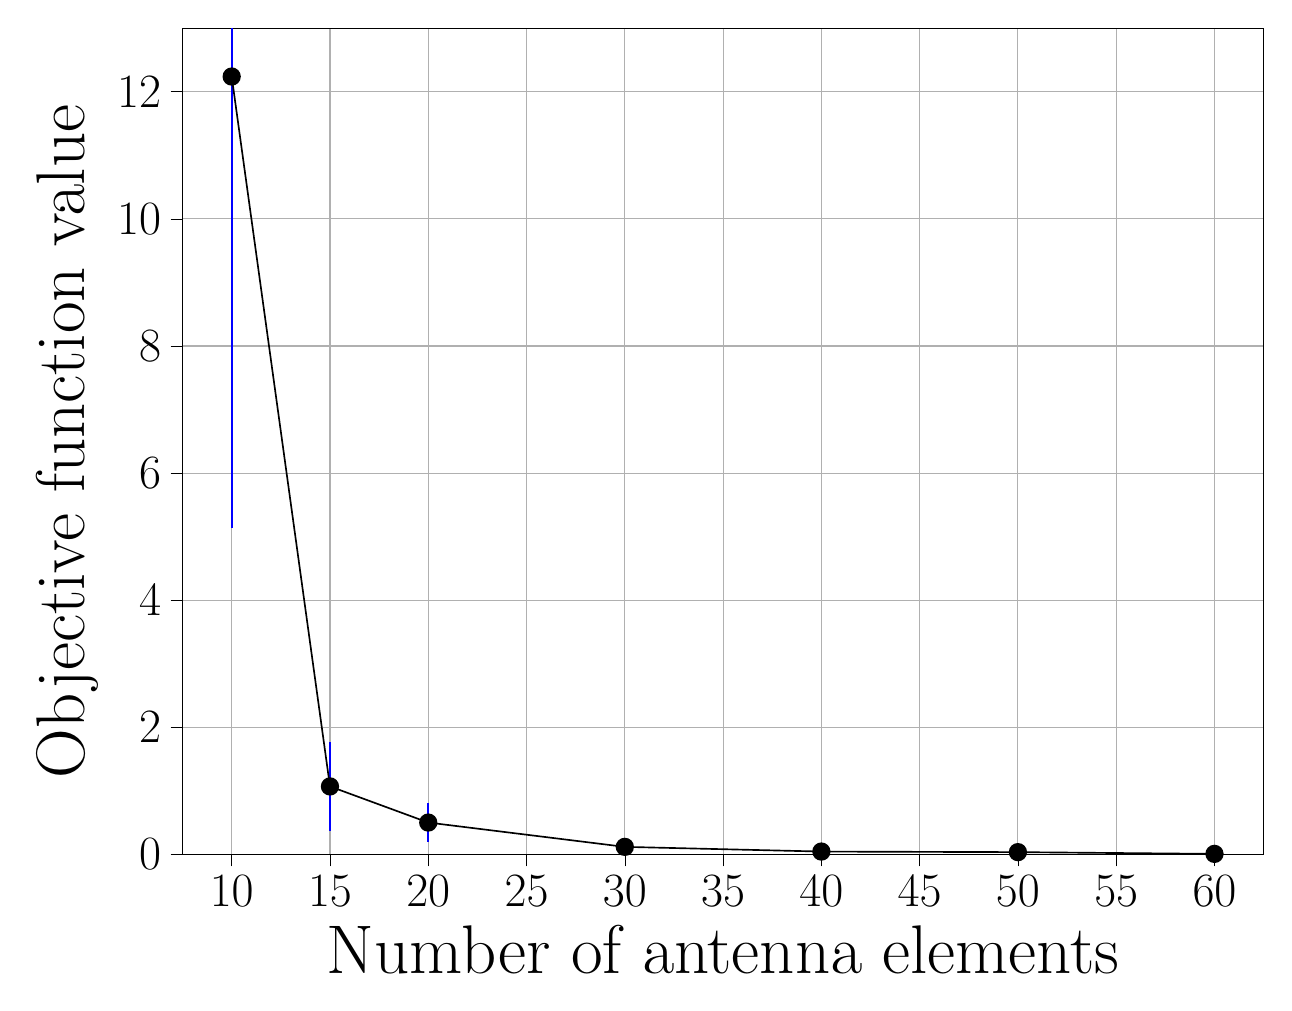
\begin{tikzpicture}

\begin{axis}[
width=6.028in,
height=4.754in,
xlabel style={font=\Huge},
ticklabel style={font=\LARGE},
ylabel style={font=\Huge},
tick align=outside,
tick pos=left,
x grid style={white!69.01960784313725!black},
xlabel={Number of antenna elements},
xmajorgrids,
xmin=7.5, xmax=62.5,
xtick style={color=black},
y grid style={white!69.01960784313725!black},
ylabel={Objective function value},
ymajorgrids,
ymin=0, ymax=13,
ytick style={color=black}
]
\path [draw=blue, thick]
(axis cs:10,5.14)
--(axis cs:10,14.34);

\path [draw=blue, thick]
(axis cs:15,0.371)
--(axis cs:15,1.771);

\path [draw=blue, thick]
(axis cs:20,0.2025)
--(axis cs:20,0.8025);

\path [draw=blue, thick]
(axis cs:30,0.1)
--(axis cs:30,0.14);

\path [draw=blue, thick]
(axis cs:40,0.036)
--(axis cs:40,0.056);

\path [draw=blue, thick]
(axis cs:50,0.037)
--(axis cs:50,0.037);

\path [draw=blue, thick]
(axis cs:60,0.0094)
--(axis cs:60,0.0094);

\addplot [semithick, black, mark=*, mark size=3, mark options={solid}]
table {%
10 12.24
15 1.071
20 0.5025
30 0.12
40 0.046
50 0.037
60 0.0094
};
\end{axis}

\end{tikzpicture}